%%%%%%%%%%%%%%%%%%%%%%%%%%%%%%%%%%%%%%%%%
% Jacobs Landscape Poster
% LaTeX Template
% Version 1.1 (14/06/14)
%
% Created by:
% Computational Physics and Biophysics Group, Jacobs University
% https://teamwork.jacobs-university.de:8443/confluence/display/CoPandBiG/LaTeX+Poster
% 
% Further modified by:
% Nathaniel Johnston (nathaniel@njohnston.ca)
%
% This template has been downloaded from:
% http://www.LaTeXTemplates.com
%
% License:
% CC BY-NC-SA 3.0 (http://creativecommons.org/licenses/by-nc-sa/3.0/)
%
%%%%%%%%%%%%%%%%%%%%%%%%%%%%%%%%%%%%%%%%%

%----------------------------------------------------------------------------------------
%	PACKAGES AND OTHER DOCUMENT CONFIGURATIONS
%----------------------------------------------------------------------------------------

\documentclass[final]{beamer}

\usepackage[scale=1.24]{beamerposter} % Use the beamerposter package for laying out the poster

\usepackage[utf8]{inputenc}

\usetheme{confposter} % Use the confposter theme supplied with this template

\setbeamercolor{block title}{fg=ngreen,bg=white} % Colors of the block titles
\setbeamercolor{block body}{fg=black,bg=white} % Colors of the body of blocks
\setbeamercolor{block alerted title}{fg=black,bg=dblue!70} % Colors of the highlighted block titles
\setbeamercolor{block alerted body}{fg=black,bg=dblue!10} % Colors of the body of highlighted blocks
% Many more colors are available for use in beamerthemeconfposter.sty

%-----------------------------------------------------------
% Define the column widths and overall poster size
% To set effective sepwid, onecolwid and twocolwid values, first choose how many columns you want and how much separation you want between columns
% In this template, the separation width chosen is 0.024 of the paper width and a 4-column layout
% onecolwid should therefore be (1-(# of columns+1)*sepwid)/# of columns e.g. (1-(4+1)*0.024)/4 = 0.22
% Set twocolwid to be (2*onecolwid)+sepwid = 0.464
% Set threecolwid to be (3*onecolwid)+2*sepwid = 0.708

\newlength{\sepwid}
\newlength{\onecolwid}
\newlength{\twocolwid}
\newlength{\threecolwid}
\setlength{\paperwidth}{48in} % A0 width: 46.8in
\setlength{\paperheight}{36in} % A0 height: 33.1in
\setlength{\sepwid}{0.024\paperwidth} % Separation width (white space) between columns
\setlength{\onecolwid}{0.22\paperwidth} % Width of one column
\setlength{\twocolwid}{0.464\paperwidth} % Width of two columns
\setlength{\threecolwid}{0.708\paperwidth} % Width of three columns
\setlength{\topmargin}{-0.5in} % Reduce the top margin size
%-----------------------------------------------------------

\usepackage{graphicx}  % Required for including images

\usepackage{booktabs} % Top and bottom rules for tables

%----------------------------------------------------------------------------------------
%	TITLE SECTION 
%----------------------------------------------------------------------------------------

\title{A new feature subset selection using bottom up clustering} % Poster title

\author{David Quesada López} % Author(s)

\institute{Computational Intelligence Group, Departamento de Inteligencia Artificial, Universidad Polit\'ecnica de Madrid, Spain} % Institution(s)

%----------------------------------------------------------------------------------------

\begin{document}

\addtobeamertemplate{block end}{}{\vspace*{2ex}} % White space under blocks
\addtobeamertemplate{block alerted end}{}{\vspace*{2ex}} % White space under highlighted (alert) blocks

\setlength{\belowcaptionskip}{2ex} % White space under figures
\setlength\belowdisplayshortskip{2ex} % White space under equations

\begin{frame}[t] % The whole poster is enclosed in one beamer frame

\begin{columns}[t] % The whole poster consists of three major columns, the second of which is split into two columns twice - the [t] option aligns each column's content to the top

\begin{column}{\sepwid}\end{column} % Empty spacer column

\begin{column}{\onecolwid} % The first column

%----------------------------------------------------------------------------------------
%	OBJECTIVES
%----------------------------------------------------------------------------------------

\begin{alertblock}{Objetivos}

Queremos seleccionar un subconjunto de variables con un método de filtrado basado en cluster jerárquico para:
\begin{itemize}
\item Reducir la dimensionalidad de nuestro dataset.
\item Conseguir un subconjunto de variables relevantes y no redundantes que sean igual o más eficientes y eficaces que el conjunto inicial.
\item Aprovechar tanto la velocidad del filtrado como la capacidad para agrupar variables del clustering. 

\end{itemize}

\end{alertblock}

%----------------------------------------------------------------------------------------
%	INTRODUCCIÓN
%----------------------------------------------------------------------------------------

\begin{block}{Introducción}

La selección del subconjunto de variables es una parte esencial en el preprocesado de los datos para reducir la dimensionalidad. Existen vários métodos para esto:

\begin{itemize}
\item Wrapper \cite{kohavi1997}, que seleccionan subconjuntos de variables en base a su precisión pero son muy costosos computacionalmente.
\item Filter \cite{peng2005}, que miden la relevancia de las variables sin mucho coste pero sin asegurar buena precisión final.
\end{itemize}

En nuestro algoritmo CFSS usaremos un método de filtrado basado en clustering jerárquico para agrupar las variables redundantes en clusters y elegir las relevantes para nuestro subconjunto.

\end{block}

%------------------------------------------------

\begin{figure}
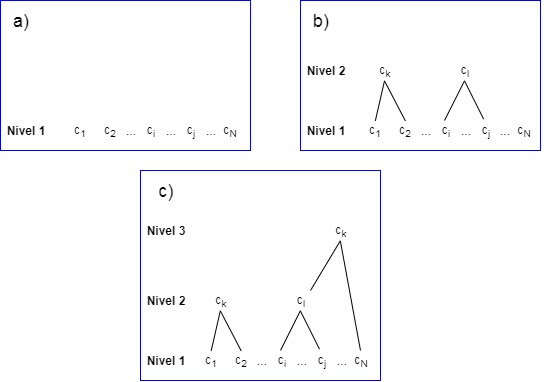
\includegraphics[width=1\linewidth]{clusterSteps.jpg}
\caption{Cluster \textit{bottom-up} de variables}
\label{fig:CL}
\end{figure}

%----------------------------------------------------------------------------------------

\end{column} % End of the first column

\begin{column}{\sepwid}\end{column} % Empty spacer column

\begin{column}{\twocolwid} % Begin a column which is two columns wide (column 2)

\begin{columns}[t,totalwidth=\twocolwid] % Split up the two columns wide column

\begin{column}{\onecolwid}\vspace{-.6in} % The first column within column 2 (column 2.1)

%----------------------------------------------------------------------------------------
%	MATERIALES
%----------------------------------------------------------------------------------------

\begin{block}{Materiales}

Para completar esta investigación se han usado los siguientes materiales:

\begin{itemize}
\item 11 datasets válidos del repositorio UCI para probar el funcionamiento de CFSS.
\item Los métodos mRMR, ReliefF y L1-LSMI para comparar el rendimiento de CFSS.
\item El algoritmo GACH para acotar el número de clusters de CFSS.
\item Un clasificador kNN en el que probar los subconjuntos devueltos por los métodos anteriores en sus respectivos datasets.
\end{itemize}

\end{block}

%----------------------------------------------------------------------------------------

\end{column} % End of column 2.1

\begin{column}{\onecolwid}\vspace{-.6in} % The second column within column 2 (column 2.2)

%----------------------------------------------------------------------------------------
%	MÉTODOS
%----------------------------------------------------------------------------------------

\begin{block}{Métodos}

El algoritmo comienza asignando cada variable a un cluster diferente (\textit{bottom-up}). Para medir la distancia entre dos variables miramos su similitud en base a su información mutua:



\end{block}

%----------------------------------------------------------------------------------------

\end{column} % End of column 2.2

\end{columns} % End of the split of column 2 - any content after this will now take up 2 columns width

%----------------------------------------------------------------------------------------
%	IMPORTANT RESULT
%----------------------------------------------------------------------------------------

\begin{alertblock}{Important Result}

Lorem ipsum dolor \textbf{sit amet}, consectetur adipiscing elit. Sed commodo molestie porta. Sed ultrices scelerisque sapien ac commodo. Donec ut volutpat elit.

\end{alertblock} 

%----------------------------------------------------------------------------------------

\begin{columns}[t,totalwidth=\twocolwid] % Split up the two columns wide column again

\begin{column}{\onecolwid} % The first column within column 2 (column 2.1)

%----------------------------------------------------------------------------------------
%	AGRUPACIÓN DE VARIABLES
%----------------------------------------------------------------------------------------

\begin{block}{Agrupación de variables}

Para agrupar las variables en clusters sigue un criterio de similaridad entre ellas, en vez de distancia, basado en la información mutua \cite{cover1991}:
  
\begin{equation}
I(f_{i},f_{j}) = \sum \sum p(f_{i},f_{j}) log \frac{p(f_{i},f_{j})}{p(f_{i})p(f_{j})}
\label{eqn:MI}
\end{equation}

Siendo $p(f_i)$ la función de distribución de esa variable. Dentro de un cluster, el centroide será la variable con una mayor información mutua con la clase. Este centroide determina la relevancia de un cluster.
\newline
\newline
Se agrupan variables en clusters hasta que no queda ningún cluster con un sólo elemento. En ese punto, se eligen qué variables se meten al subconjunto final: se empieza a añadir desde los clusters más relevantes. De un mismo cluster se pueden meter más de una, y de clusters menos relevantes que un mínimo establecido se pueden ignorar sus variables.

\end{block}

%----------------------------------------------------------------------------------------

\end{column} % End of column 2.1

\begin{column}{\onecolwid} % The second column within column 2 (column 2.2)

%----------------------------------------------------------------------------------------
%	RESULTADOS
%----------------------------------------------------------------------------------------

\begin{block}{Results}

\begin{figure}

\includegraphics[width=0.8\linewidth]{placeholder.jpg}
\caption{Figure caption}
\end{figure}

Nunc tempus venenatis facilisis. Curabitur suscipit consequat eros non porttitor. Sed a massa dolor, id ornare enim:

\begin{table}
\vspace{2ex}
\begin{tabular}{l l l}
\toprule
\textbf{Treatments} & \textbf{Response 1} & \textbf{Response 2}\\
\midrule
Treatment 1 & 0.0003262 & 0.562 \\
Treatment 2 & 0.0015681 & 0.910 \\
Treatment 3 & 0.0009271 & 0.296 \\
\bottomrule
\end{tabular}
\caption{Table caption}
\end{table}

\end{block}

%----------------------------------------------------------------------------------------

\end{column} % End of column 2.2

\end{columns} % End of the split of column 2

\end{column} % End of the second column

\begin{column}{\sepwid}\end{column} % Empty spacer column

\begin{column}{\onecolwid} % The third column

%----------------------------------------------------------------------------------------
%	CONCLUSION
%----------------------------------------------------------------------------------------

\begin{block}{Conclusion}

Nunc tempus venenatis facilisis. \textbf{Curabitur suscipit} consequat eros non porttitor. Sed a massa dolor, id ornare enim. Fusce quis massa dictum tortor \textbf{tincidunt mattis}. Donec quam est, lobortis quis pretium at, laoreet scelerisque lacus. Nam quis odio enim, in molestie libero. Vivamus cursus mi at \textit{nulla elementum sollicitudin}.

\end{block}

%----------------------------------------------------------------------------------------
%	Artículo real
%----------------------------------------------------------------------------------------

\begin{block}{Artículo real}

Dehghan Z., Mansoori E. G. (2016). A new feature subset selection using bottom-up clustering. \textit{Pattern Analysis and Applications}, 1-10.

\end{block}

%----------------------------------------------------------------------------------------
%	Referencias
%----------------------------------------------------------------------------------------

%\setbeamercolor{block title}{fg=red,bg=white} % Change the block title color

\begin{block}{Referencias}
\nocite{*} % Insert publications even if they are not cited in the poster
\small{\bibliographystyle{plainnat}}
\begin{thebibliography}{}

\bibitem{cover1991}
Cover TM, Thomas JA (1991) Elements of information theory. Wiley, New York

\bibitem{kohavi1997}
Kohavi R, John GH (1997) Wrapper for feature subset selection. Artif Intell 97(1–2):273–324

\bibitem{peng2005}
Peng H, Long F, Ding C (2005) Feature selection based on mutual information: criteria of max-dependency, max-relevance, and min-redundance. IEEE Trans Pattern Anal Mach Intell 27(8):1226–1238

\end{thebibliography}

\end{block}

%----------------------------------------------------------------------------------------
%	CONTACT INFORMATION
%----------------------------------------------------------------------------------------

%\setbeamercolor{block alerted title}{fg=black,bg=norange} % Change the alert block title colors
%\setbeamercolor{block alerted body}{fg=black,bg=white} % Change the alert block body colors

\begin{center}
\begin{tabular}{ccc}

\includegraphics[width=0.4\linewidth]{logoUPM.jpg} 
\end{tabular}
\end{center}

%----------------------------------------------------------------------------------------

\end{column} % End of the third column

\end{columns} % End of all the columns in the poster

\end{frame} % End of the enclosing frame

\end{document}
